\documentclass{sciposter}

\usepackage[brazil]{babel}
\usepackage[utf8]{inputenc}
\usepackage[centertags]{amsmath}
\usepackage{hyperref,amsfonts,multirow,multicol}
\hypersetup{pdfpagelayout=SinglePage}
\usepackage{graphicx,colortbl}
\usepackage{geometry}
\geometry{paperwidth=90cm,paperheight=100cm,centering,
textwidth=77cm,textheight=87cm,left=3cm,top=3cm}
\usepackage{braket}
\usepackage{multicol}
\usepackage{wrapfig}
\pagestyle{plain}
\frenchspacing

%%Definindo cores
\definecolor{BoxCol}{RGB}{44,54,181} %azul

%%Define o caminho das figuras, válido somente para o comando \includegraphics
\graphicspath{{imagens/}}


%%Transformando tudo em branco
\renewcommand{\thesection}{\textcolor{white}{\arabic{section}}}
\renewcommand{\thesubsection}{\textcolor{white}{\arabic{section}.\arabic{subsection}}}
\addto\captionsbrazil{\renewcommand{\bibname}{\textcolor{white}{Refer\^encias}}}

%%Definindo de novos comandos

\newcommand{\tituloA}[1]{\emph{\textbf{\color{white}{#1}}}}
\newcommand{\tituloB}[1]{\emph{\textbf{\color{blue}{#1}}}}
\newcommand{\R}{\mathbb{R}}




\begin{document}



%%Titulo do Trabalho
 \colorbox{BoxCol}{
  \begin{minipage}{\textwidth}
   \color{white}{
    \begin{center}
     \huge{\textbf{\vspace{1cm} \\
       UFRJ NA PRAÇA
       \vspace{1cm} \\}}
     \end{center}
    }
  \end{minipage}
  }

\qquad



%%Autores, Instituto, E-mails
\title{} % n\~ao delete
\author{\Huge{\textbf{Criptografia Quântica}}}
%%\institute{Laboratório de Óptica Quântica - Instituto de Física - UFRJ}
%%\email{\texttt{otaviocals@if.ufrj.br - }}
%%\leftlogo[0.6]{logo} %logotipo da universidade

\qquad

  \begin{minipage}{\textwidth}
   \begin{flushleft}

    \raisebox{1cm}{\hspace{1cm}
\includegraphics[width=6cm]{minerva}}\raisebox{5cm}{\hspace{-6.5cm}\maketitle}\raisebox{4cm}{\hspace{-6.5cm}
\includegraphics[width=8cm]{qrio}}

   \end{flushleft}
  \end{minipage}




%%\noindent\maketitle %gera titulo

%% Jornada, Congresso, Assembleia, etc
\colorbox{BoxCol}{
  \begin{minipage}{\textwidth}
   \color{white}{
    \begin{center}
      \vspace{0.5cm}
      %digite o nome do congresso aqui
      \Large{\textbf{\vspace{1cm} \\ Laboratório de Óptica Quântica - Instituto de Física - UFRJ \vspace{1cm} \\}}
      \vspace{0.5cm}
    \end{center}
    }
  \end{minipage}
}

\quad



%Numero de Colunas
\begin{multicols*}{2}{
\raggedcolumns

%Paragrafo.
\setlength{\parindent}{2em}

%%Primeira Secao
\section*{\tituloA{\color{white}{\Large {Segurança? Codificação? Cripto-quê???}}}}
\par


\begin{wrapfigure}[4]{l}{8cm}
    \vspace{-3cm}
    
\includegraphics[width=10cm]{criptografia}
\end{wrapfigure}

\vspace{3cm}
\Large\textbf{Criptografia}: Conjunto de técnicas para codificar mensagens, utlizando chaves criptográficas, de tal forma que apenas o emissor e o receptor dessas as consigam ler.\\

\vspace{1cm}
\hspace{3cm}
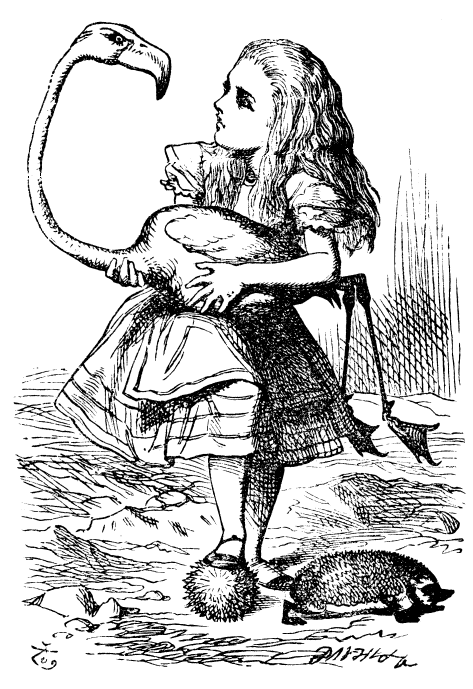
\includegraphics[width=5cm]{alice2}
\hspace{15.5cm}
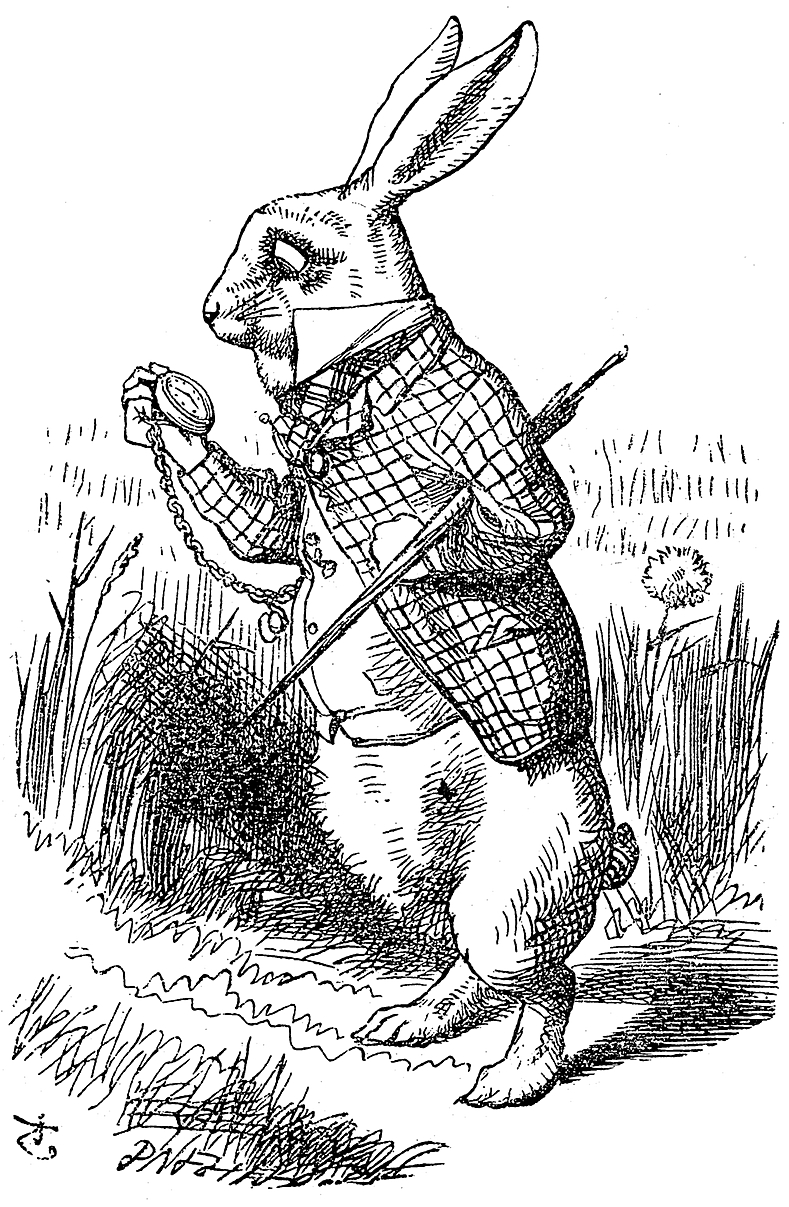
\includegraphics[width=5cm]{bob2}\\

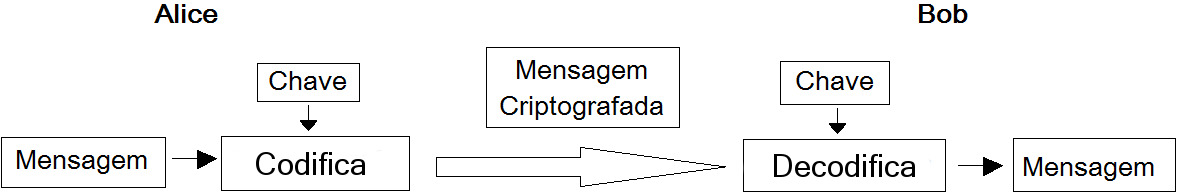
\includegraphics[width=33cm]{classiccript}

\vspace{1cm}
\par Atualmente, métodos criptográficos podem ser encontrados em diversas aplicações, como por exemplo, caixas eletrônicos, aplicativos de smartphones e redes sociais.

\vspace{1cm}
\hspace{6cm}
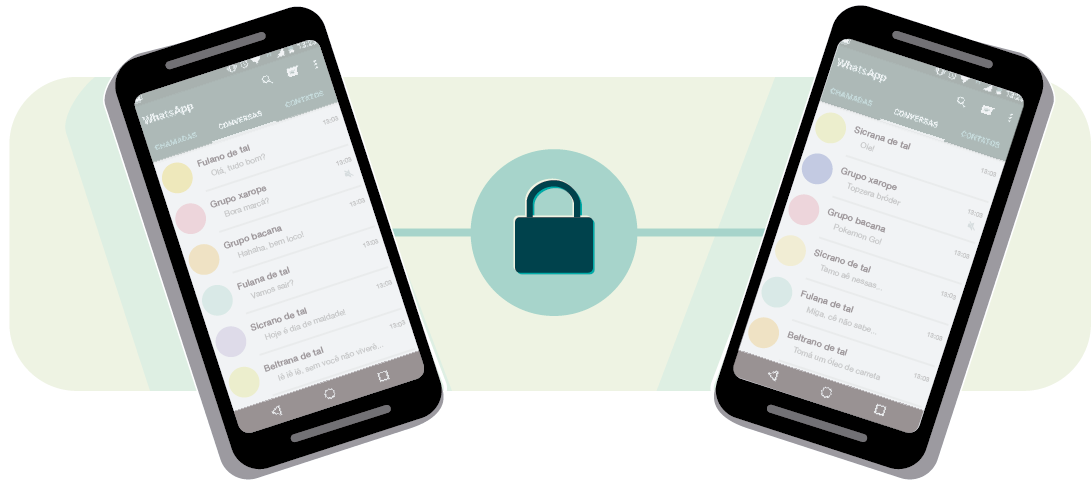
\includegraphics[width=21cm]{cripto_cell}





\section*{\tituloA{\color{white}{\Large{A eterna luta do Gato e o Rato}}}}
\par Desafio da criptografia: Proteger a chave criptográfica contra o acesso de \textbf{espiões}.

\hspace{11.5cm}

\includegraphics[width=10cm]{spy}

\par Para solucionar esse problema, físicos, matemáticos e cientistas da computação estudaram novas formas de criptografia, criando a área conhecida hoje como Criptografia Quântica.


\vfill
\columnbreak


\section*{\tituloA{\color{white}{\Large{Gatos, Lasers e Criptografia}}}}

\begin{wrapfigure}[5]{r}{14cm}
    \vspace{-1cm}
    \hspace{-2.5cm}
    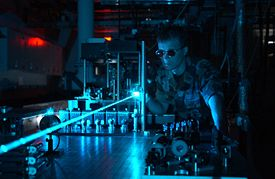
\includegraphics[width=16cm]{laser}
\end{wrapfigure}

\vspace{1cm}
\textbf{Criptografia Quântica}: protocolos que, baseados na mecânica quântica, garantem a transmissão de chaves de forma segura, independente do poder computacional de um possível hacker.

\vspace{1cm}
\par Nossa implementação busca realizar transmissões quânticas de chave à grandes distâncias de forma rápida e eficiente. A seguir podemos ver algumas fotos do nosso experimento.

\vspace{1cm}
\hspace{1cm}
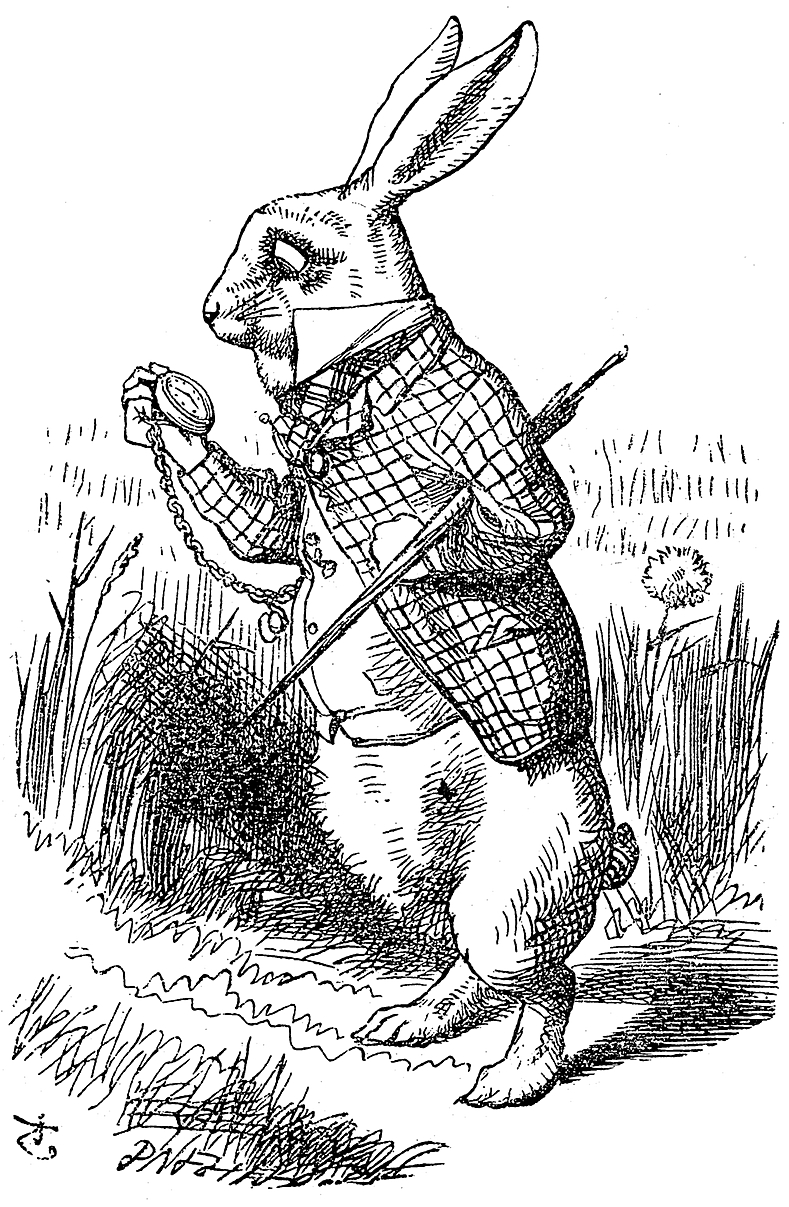
\includegraphics[width=15cm]{bob}
\hspace{0.5cm}
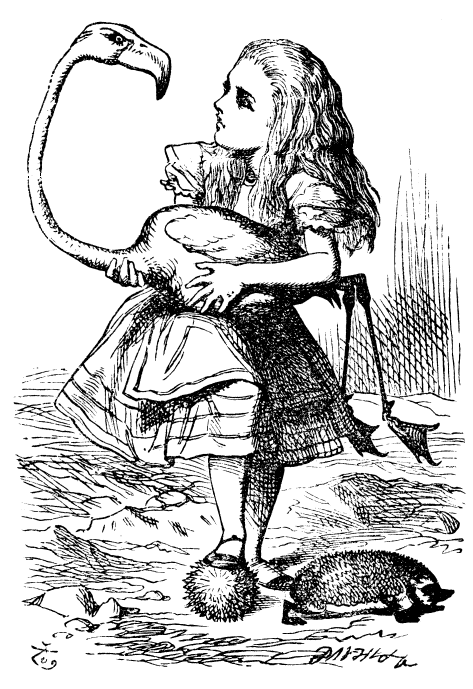
\includegraphics[width=15cm]{alice}

\vspace{1cm}
\hspace{8.75cm}
\includegraphics[width=15cm]{new_alice}



\section*{\tituloA{\color{white}{\Large{Ao Infinito e Além!}}}}

\par Atualmente existem centros de pesquisas e empresas explorando criptografia quântica em diversos lugares do mundo.\\

\hspace{4cm}
\vspace{2cm}

\includegraphics[width=10cm]{idq}
\hspace{4cm}
\vspace{-4cm}

\includegraphics[width=15cm]{sequrenet}\\

\vspace{2cm}
\par Nosso estudos buscam gerar experiência e desenvolvimento nacional e, junto ao efervescente cenário brasileiro de segurança da informação, tornar o Brasil uma referêrencia na área.


}
\end{multicols*}



\end{document}
